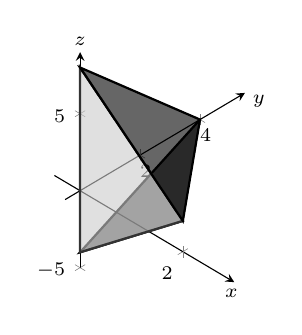
\begin{tikzpicture}[>=stealth]
\begin{axis}%
[width=175pt,height=200pt,
tick label style={font=\scriptsize},%axis on top,
			axis lines=center,
			view={45}{35},
			name=myplot,
			%xtick=\empty,
			%ytick=\empty,
			%ztick=\empty,
			%extra x ticks={1},
			%extra x tick labels={$a$},
			%extra y ticks={1},
			%extra y tick labels={$a$},
			%extra z ticks={1},
			%extra z tick labels={$h$},
			ymin=-.5,ymax=5.5,
			xmin=-.5,xmax=3,
			zmin=-5, zmax=9,
			every axis x label/.style={at={(axis cs:\pgfkeysvalueof{/pgfplots/xmax},0,0)},xshift=-1pt,yshift=-4pt},
				xlabel={\scriptsize $x$},
			every axis y label/.style={at={(axis cs:0,\pgfkeysvalueof{/pgfplots/ymax},0)},xshift=5pt,yshift=-3pt},
				ylabel={\scriptsize $y$},
				every axis z label/.style={at={(axis cs:0,0,\pgfkeysvalueof{/pgfplots/zmax})},xshift=0pt,yshift=4pt},
				zlabel={\scriptsize $z$}
			]


%\draw [{\colortwo},thick] (axis cs: 0,4,0) -- (axis cs: 2,4,-6) -- (axis cs: 2,0,2);


%\addplot3[domain=0:2,,y domain=0:4,surf,%fill=white,
%colormap={mp2}{\colormapplaneone},opacity=.6,faceted color=black!40,samples=2,samples y=2,very thin,z buffer=sort] {3*x+y-4};

\draw [{\coloronefill},thin,fill={\coloronefill},opacity=.6] (axis cs: 0,4,0) -- (axis cs: 0,0,-4) -- (axis cs: 2,0,2)--cycle;


\draw [{\colorone},thick] (axis cs: 0,4,0) -- (axis cs: 0,0,-4) -- (axis cs: 2,0,2);

\filldraw [{\colortwofill},thin,fill={\colortwofill},opacity=.6] (axis cs: 0,4,0) -- (axis cs:0,0,8) -- (axis cs: 2,0,2) --cycle;



\draw [black!20,thin,fill=black!20,opacity=.6] (axis cs: 0,0,8) -- (axis cs: 2,0,2) -- (axis cs:0,0,-4) -- cycle;

\draw [black!80, thick] (axis cs: 0,0,8) -- (axis cs: 2,0,2) -- (axis cs:0,0,-4)--cycle;

\draw [{\colortwo},thick] (axis cs: 0,4,0) -- (axis cs:0,0,8) -- (axis cs: 2,0,2) --cycle;
%\addplot3[domain=0:2,,y domain=0:4,surf,%fill=white,
%colormap={mp2}{\colormaptwo},opacity=.6,faceted color=black!40,samples=2,samples y=2,very thin,z buffer=sort] {8-3*x-2*y};

%\draw [{\colorone},thick] (axis cs: 2,0,2) -- (axis cs: 2,4,6) -- (axis cs: 0,4,0);

%\draw [dashed,thick] (axis cs: 2,0,2) -- (axis cs: 0,4,0);



\end{axis}


\end{tikzpicture}












